\part{Sejlskibsepoken}

\begin{figure}
\centering
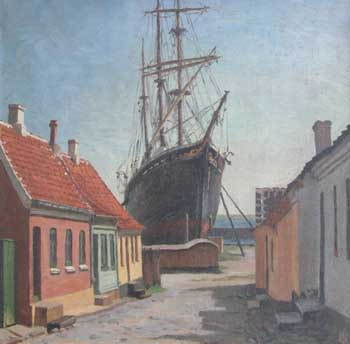
\includegraphics{images/epoker_sejlskibe.jpg}
\caption{\{1\}}
\end{figure}

\begin{intro}
%\sFram{pageIntro}{
I sejlskibsepoken blev de fleste varer transporteret rundt i verdenen med
sejlskibe. Industrialiseringen betød, at der blev behov for at
transportere flere og flere varer mellem byerne og mellem
landdistrikterne og havne.%}
\end{intro}

\begin{figure}
\centering
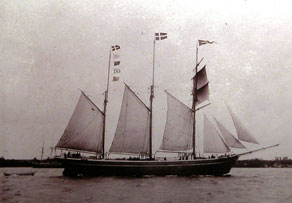
\includegraphics{images/sejlskibe_indledning-nanna.jpg}
\caption{Nanna af Svendborg}
\end{figure}

Sejlskibe udgjorde rygraden af den danske handelsflåde helt frem til
omkring 1900. Man brugte oftest søvejen, når varer skulle fra et sted
til et andet. Det var mange gange nemmere at sejle end at benytte
bumpede og mangelfulde landeveje, og så kunne et skib flytte langt mere
gods end en hestevogn. Det blev på den måde billigere at transportere
varer og mennesker over havet i stedet for over land. De fleste byer lå
da også ved en kyst med nem adgang til søtransport.

1870 var industrialiseringen så småt begyndt herhjemme. Jernbanenettet
blev udbygget, fabrikker blev opført, og befolkningen voksede meget
hurtigt på grund af bedre levevilkår. Der blev derfor et stadigt større
behov for at transportere varer rundt mellem byerne og mellem
landdistrikter og havne. Til at dække behovet søsatte man stadigt flere
skibe, og selv om dampskibet var opfundet, byggede man stadigvæk mange
sejlskibe. De var længe billigere både at bygge og at sejle med.
Ulemperne var dog flere. Sejlskibene var afhængige af vind og vejr.
Blæste der ingen vind, kunne skibet ikke sejle. Blæste der for meget
vind, kunne skibet være svært at styre. Og det risikerede at gå på grund
eller måske at blive knust mod en klippeside.

\begin{figure}
\centering
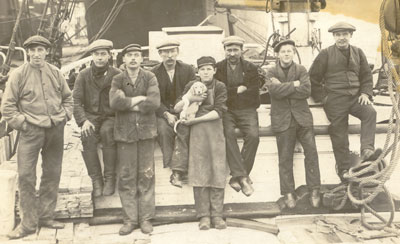
\includegraphics{images/sejlskibe_indledning-skibsh.jpg}
\caption{Besætning på et sejlskib. Drengen holder skibshunden.}
\end{figure}

Sejlskibe var heller ikke helt så punktlige, og så kunne det tage lang
tid at \textbf{laste}\footnote{\textbf{Laste} er, når varer eller gods
  tages om bord på et skib.} og \textbf{losse}\footnote{\textbf{Losse}
  er, naar varer eller gods tages fra borde paa et skib.} skibet. Det
kunne også være temmelig risikabelt at sejle med disse sejlskibe. Mange
sømænd forsvandt sporløst, hvis et skib for eksempel ramte et isbjerg
eller kæntrede, når lasten forskubbede sig i hård søgang. Alligevel
kunne det betale sig at søsætte nye sejlskibe. Hver gang skipperen eller
kaptajnen afleverede en ladning sikkert i havn, fik skibets ejere oftest
et fint overskud, selvom priserne naturligvis svingede, og nogle år var
bedre end andre. Mange redere brugte overskuddet til at bygge nye skibe.
På den måde tjente de flere penge - og så kunne de købe endnu flere
skibe. Nogle områder og byer i Danmark specialiserede sig i
sejlskibssøfarten. Den var ganske vist risikabel, men gav også mange
mennesker brød på bordet hver dag. Et af disse områder lå i Det
sydfynske Øhav.

\chapter{Livet på land}

\emph{``Vi legede med små træskibe og planker om sommeren og vadede
rundt og skubbede til dem, hvis det ikke gik stærkt nok.''}

\begin{figure}
\centering
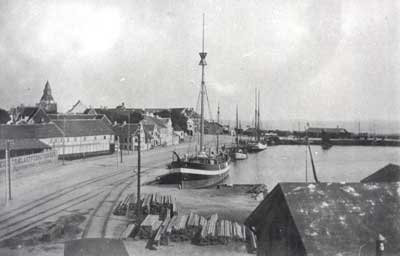
\includegraphics{images/sejlskibe_tema-1-toemmer.jpg}
\caption{Tømmerstabler på Faaborg Havn.}
\end{figure}

På havnen var der altid noget at se, når de store sejlskibe kom ind.
Hestevogne hentede de mange varer, som skibene havde med. Og søfolkene
fortalte historier fra fremmede lande. Havnen var spændende og satte
fantasien i gang. Ville man ud at opleve verden, måtte man sejle af
sted, for der var ingen andre muligheder. Sejlskibene satte derfor gang
i drømmen om den store verden. Voksede børnene op i en søfartsby fjollet
eller i en \textbf{havneby}\footnote{\textbf{Havneby} er en by med en
  større havn}, var det ikke usædvanligt, at de legede på havnen, selv
om det ikke altid var ufarligt.

\begin{figure}
\centering
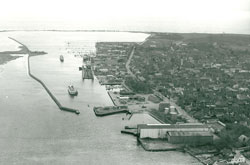
\includegraphics{images/sejlskibe_tema-1-marstal.jpg}
\caption{Marstal var en af de byer, der i 1700-tallet blev en
betydningsfuld søfartsby.}
\end{figure}

\sFram{showBlue}{
    \subsection{Søfartsby}

    En søfartsby var en by, der lå ved vandet. I byen levede befolkningen mest
    af søfarten. I Danmark lå mange af disse søfartsbyer på øer, hvor sejlads
    under alle omstændigheder var vigtig. I søfartsbyerne var der en stor del
    af den mandlige befolkning, som sejlede. De kom ofte hjem om vinteren,
    inden stormene blev for kraftige, og isen lukkede farvandene. Om vinteren
    var familien derfor samlet, og man fik ordnet de praktiske ting. Det var
    gerne i denne periode, at giftermål blev indgået og pengene gjort op. Der
    blev festet og levet, inden isen brød op, og mændene igen skulle ud på
    bølgerne. I nogle søfartsbyer blev der udviklet forskellige skikke, der
    kunne være meget anderledes end dem, man kendte fra andre byer.

    Når mændene var ude at sejle, tog kvinderne sig af de økonomiske sager og
    alt det, der havde med hjemmet at gøre. At være sømandskone var noget helt
    specielt på linje med det at være sømand.

    Nogle rigtige og vigtige søfartsbyer herhjemme var Marstal på Ærø, Troense
    på Tåsinge, Dragør på Amager, Nordby og Sønderho på Fanø. Der var også
    mange sejlskibe og søfolk i byer som Faaborg, Ærøskøbing, Svendborg og
    Rudkøbing. Tilsammen udgjorde det sydfynske øhav et center for sejl-skibe,
    hvor der i sejlskibstiden var omkring 1/3 af alle danske sejlskibe.
}

\emph{''Undertiden legede vi på tømmerstablerne på Faaborg Trælast. Vi
klatrede op og sprang fra den ene til den anden. Når så
\textbf{havnefogeden}\footnote{\textbf{Havnefoged} er en mand, der er
  ansat til at styre havnen.} kom, fik vi øretæver, hvis han fik fat i
nogen. Ellers var vi meget på havnen. Jeg måtte ikke løbe til havnen
uden at få lov. Men jeg løb sgu derned alligevel og så vankede der
stryg, hvis far opdagede det. Det var alle skibene i havnen der trak, og
vi kom i snak med skibsdrengene, der kunne fortælle historier og vise
uartige billeder. Der var ikke ret mange drenge, der holdt sig dernede
fra.''}

\emph{''Vi drillede havnefogeden. Det var gamle Noack. Når havnefogeden
var efter os, så kravlede vi ned mellem pælene og ind på
\textbf{glaciset}\footnote{\textbf{Glacis} er en stenvæg, der går skråt
  ud i vandet.}, så kunne han sgutte få fat i os. Vi lavede mange numre,
og så kom Noack hen til den gamle og sagde: De satans knægte!''}

Den daglige færden på havnen gav mulighed for at hjælpe mændene på
skibene. Hvis man var rigtig heldig, kunne man få lov at kravle op i
skibenes master.

\emph{''Der kom mange 3-mastere til \textbf{Bagenkop}\footnote{\textbf{Bagenkop}
  er et fiskerleje på sydspidsen af Langeland.} med kul. Så ville vi jo
gerne op at hjælpe til, sejlene skulle tørres osv. Vi fik lov på den
betingelse, at vi skulle hente hver 10 spande vand om dagen og komme
vandfad på dækket. Hvis vi så hentede 10 spande vand om dagen, så måtte
vi kravle op i riggen.''}

\sFram{showBlue}{
    \subsection{Riggen}

Rigningen er den del af sejlskibet, som sejlene hejses op i. Rigningen er bygget op omkring skibets master og består af en masse tovværk. At kravle til tops i rigningen var et farligt og besværligt arbejde og derfor ikke altid populært blandt søfolkene.
}

\begin{figure}
\centering
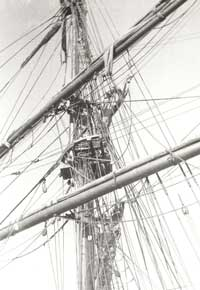
\includegraphics{images/sejlskibe_tema-1-riggen.jpg}
\caption{Riggen på et sejlskib.}
\end{figure}

\emph{''Vi drenge vi lå jo og kravlede i rigningen på de skibe, der
lagde op om vinteren. Vi skulle se hvem der kunne komme hurtigst op og
lægge sig på maven oppe på fløjknappen. Ja Gud fri mig vel \(\ldots\) at
der ikke skete en ulykke! Vi var som aber dengang. Det var noget alle
drenge gjorde.''}

Man fik et naturligt forhold til at sejle, hvis man voksede op ved
vandet.

\emph{''Vi var dårligt nok kommet ned på havnen, så lå vi nede i en
jolle og roede jo. Ja der var jo altid nogen større med, som havde
forstand på det, indtil vi andre havde fået sat det rigtigt sammen, så
kom det. Det var både med sejljoller og rojoller.''}

Nogle blev indført i jollelivet af nødvendighed. Ikke alle steder var
der råd til at lade børnene bruge tid i skolen.

\emph{''Vi boede i et fiskerleje nord for \textbf{Assens}\footnote{\textbf{Assens}
  er en by på Fyn.} -- Aborg Strand. Min far havde temmelig gode
kundskaber, og han søgte skolevæsenet om, at vi ikke kunne slippe for at
gå i skole, for vi var nødt til at være hjemme for at hjælpe dem, imod
at han underviste os, og vi mødte hvert år til eksamen sammen med de
andre børn og kunne klare os. Når vi lå derude og slæbte ålevåd om
natten, så lå vi og drev sådan som omstændighederne var i tre kvarter
til en time -- så sad vi rigtignok nede i logaret og terpede, så stak
den gamle lige hovedet op af kappen en gang imellem for at se om der var
noget usædvanligt. For ellers så sad han og terpede med os dernede. Om
det så var tysk, så kunne vi det.''}

\sFram{showBlue}{
    \subsection{Jollen}

En jolle er et af de mindste fartøjer, man kan sejle i. Jollerne bliver enten
drevet frem af sejl eller årer. Man brugte jollerne til mange forskellige
mindre opgaver. Skulle man ud til et skib, der lå for anker, brugte man jollen
til at ro ud til det. Joller var også det foretrukne transportmiddel til
kortere ture mellem øer eller måske i havne og lignende. Større joller havde
fiskerne glæde af, når de skulle røgte garn eller ruser. Joller blev desuden
brugt som redningsbåde, selv om de ikke var særligt egnede til det. Indtil
1960’erne var det bådebyggerne, som lavede de fleste joller. De blev bygget i
hånden og var lavet i træ. Senere blev jollerne bygget af glasfiber, og
en del af disse var masseproducerede. I dag er de fleste joller forsynet med
motor, og man ser kun sjældent en jolle, der bliver roet.
}

I søfartssamfundene lå det ligefrem i luften, at søen ventede forude.

\emph{``Selvfølgelig færdedes vi børn ved havnen, så snart der var
lejlighed til det, og tumlede os i joller, og dengang var der jo en hel
del sejlskibe hjemmehørende her i \textbf{Ærøskøbing}\footnote{\textbf{Ærøskøbing}
  er en by på Ærø.} og det var jo en begivenhed at komme ned at se, hvis
de kom hjem om efteråret og havde været ude siden marts måned. Så kom de
gerne hjem med en ladning kul eller \textbf{ballastet}\footnote{\textbf{Ballast}
  er sten eller sand, som man puttede i bunden af et tomt skib, så det
  ikke væltede.} hjem for at lægge op, og så var vi jo ved jollen, når
de var fortøjet og roede omkring i den. Og selvfølgelig fik vi lyst til
søen. I \textbf{Marstal}\footnote{\textbf{Marstal} er en søfartsby på
  øen Ærø, der ligger syd for Fyn.} var det jo sådan, at hvis en dreng
ikke ville til søs, når han var konfirmeret, så var det jo ikke nogen
rigtig dreng. De få, der kom i håndværkslære eller sådan noget, de var
ikke rigtig anset, og der var noget af det samme her, men ikke så
udtalt.''}

\begin{figure}
\centering
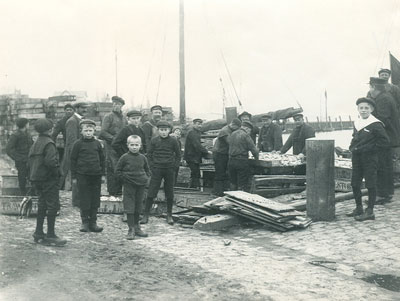
\includegraphics{images/sejlskibe_tema-1-boern.jpg}
\caption{Børn ved havnen.}
\end{figure}

Nogle piger syntes også, at havnen var et spændende sted. Men
omgivelserne var ikke altid klar til at lade piger løbe rundt på havnen.

\emph{''Jeg har været en ti til tolv år, da jeg var sluppet ned på
havnen og ivrigt iagttog en skonnert blive losset. Jeg havde hørt i
skolen, at der var nogle tyrkere med om bord, og dem ville jeg gerne se,
hvordan de så ud. De drejede det tunge lossespil med de tunge kurve på.
Jeg stod bare i cirka 15 meters afstand og kiggede på dette. Det har
ikke varet længere end et kvarter eller tyve minutter. Længere tid havde
jeg ikke til min rådighed. Jeg havde en gammel dame at gå byærinder for
efter skoletid. Om aftenen mødte en tante op. Oh, ve, nogen havde bedt
hende gå til min mor og fortælle, at jeg løb på havnen og var ude efter
fremmede søfolk. Jeg havde en fornuftig mor, som bad mig om at blive
derfra, så hun kunne blive fri for sådanne sladderhistorier, men jeg kom
aldrig på havnen alene mere.''}

\begin{figure}
\centering
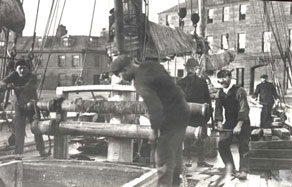
\includegraphics{images/sejlskibe_tema-1-lossespil.jpg}
\caption{Et lossespil i brug.}
\end{figure}

\sFram{showBlue}{
    \subsection{Lossespil}
Lossespil var en mekanisme, som gjorde det nemmere at laste og losse skibet - altså at putte varer ned i skibet eller at tage varerne op fra skibet. Når man drejede håndtagene på lossespillet, trak man samtidig i et stykke tov, der var forbundet med lossehjulet. På lossehjulet var der en krog. På den kunne man fastgøre kurve eller kasser fyldt med gods. Det tog en uge at laste et skib med et hånd-drevet lossespil. Efterhånden blev lossespillene motoriserede med små damp- eller benzinmotorer. I dag bruger man ikke lossespil mere, men faste krananlæg eller mobilkraner.
}

\chapter{Far-vel}

\emph{``Jeg var lige konfirmeret og så skulle jeg ud med den gamle
Petersen, det var vores nabo. Han boede ved siden af far og mor, og det
var vist aftalt længe før jeg blev konfirmeret.''}

\begin{figure}
\centering
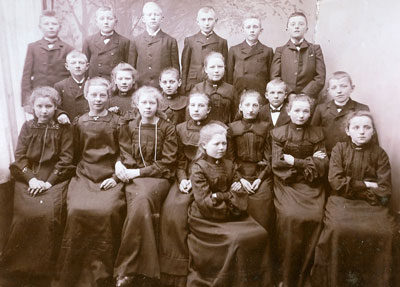
\includegraphics{images/sejlskibe_tema-2-konfirmand.jpg}
\caption{Konfirmander fra 1914.}
\end{figure}

I \textbf{sejlskibstiden}\footnote{\textbf{Sejlskibstid} er dengang,
  sejlskibene sejlede.} havde man ikke mulighed for at vælge mellem
uddannelser og beskæftigelse som i dag. Drengene kom meget ofte til at
lave det samme som faderen, mens pigerne skulle lære at holde hus ved at
tjene på gårdene eller i større husholdninger. Her skulle de være, til
de var \textbf{giftemodne}\footnote{\textbf{Giftemoden} er, når man er
  gammel nok til at blive gift.}. Konfirmationen var et afgørende skel.
Det omgivende samfund anså herefter én for at være klar til
arbejdslivet. Når man blev konfirmeret, gik der ikke længe, før leg blev
til alvor. Familierne var børnerige og havde som regel ikke ret mange
penge. Når barnet blev sendt af sted, var der en mund mindre at mætte.
Hvis man var dreng i et søfartssamfund, eller hvis ens familie var
beskæftiget i \textbf{søfartserhvervet}\footnote{\textbf{Søfartserhverv}
  er de jobs, som har forbindelse med skibe.}, så var der gode chancer
for, at man selv skulle til søs. Tradition spillede en stor rolle, og
mange gange var det allerede aftalt på forhånd, hvilket skib den unge
skulle sejle med. Nogle gange kunne det gå hurtigt, og før konfirmanden
vidste af det, kunne han være på vej til skibet.

\emph{''Konfirmationsfesten skulle være om onsdagen, da vi skulle til
alters, og \textbf{da var jo lagt stort i kakkelovnen}\footnote{\textbf{``Lagt
  i kakkelovnen''} er et udtryk for optræk til ballade.}. De skulle jo
være der alle sammen, når vi kom hjem fra den kirkehistorie der, og
skulle spise, og det gik fint med det, og så der klokken 5 om
eftermiddagen, da kom der sgu et telegram at jeg skulle rejse klokken 5.
Jeg havde fået \textbf{hyre}\footnote{\textbf{Hyre} betyder løn.}.''}

Arbejdsaftaler med skipperen eller ejeren af skibet var tit indgået på
forhånd, men før man kunne komme om bord, skulle man lige ses an.

\emph{''Jeg gik med min bedstemor derned, og hun spurgte, om han havde
brug for en dreng. Ja, det har vi, sagde han, er det ham der? Ja, det
var det jo. Ja vi kan godt prøve at tage ham med. Og så skulle jeg have
10 kr. om måneden, og hvis jeg så duede til noget skulle jeg have 15
kr.''.}

I søfartssamfund blev konfirmationen afholdt tidligere, så drengene
kunne nå at sejle ud med skibene, lige så snart \textbf{\emph{isen}}
begyndte at smelte i slutningen af marts eller i begyndelsen af april:

\begin{figure}
\centering
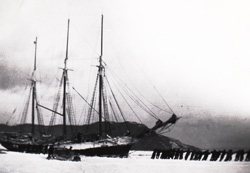
\includegraphics{images/sejlskibe_tema-2-isen.jpg}
\caption{En mergelspiger til splejsning af reb, og åbning/lukning af
sjækler.}
\end{figure}

\sFram{showBlue}{
    \subsection{Isen}
I 1800-tallet og første halvdel af 1900-tallet var klimaet koldere end i dag. Det betød, at de indre farvande ofte frøs til med is. Isen gjorde det umuligt at sejle med sejlskibe. Farvandene begyndte at ise til i løbet af januar, og i nogle år skulle man helt hen til april, før man kunne genoptage sejladsen. Oftest kunne sejlskibene dog sejle ud i løbet af marts måned.}

\emph{''Vi havde altid konfirmation 14 dage før andre havde. Så sejlede
vi til \textbf{Marstal}. De skibe der havde været hjemme og overvintre
og blev repareret om vinteren, de skulle gerne ud senest i april og så
skulle konfirmationen være overstået først. Det var
\textbf{hyrebasser}\footnote{\textbf{Hyrebasser} er folk, der ledte
  efter mænd og drenge, som kunne få job på skibene}, det kaldte vi dem
dengang, altså privatfolk, der \textbf{forhyrede}\footnote{\textbf{Forhyrede}
  er ansatte, som gør tjeneste på et handelsskib mod betaling.} søfolk.
De havde gerne sådan en lille søudrustningsforretning ved siden af med
olietøj og søstøvler og forskellige knive, hvad en sømand skulle have,
merlespir og sejlhandsker og sådan.''}

\begin{figure}
\centering
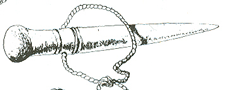
\includegraphics{images/sejlskibe_tema-2-merlespige.png}
\caption{En mergelspiger til splejsning af reb, og åbning/lukning af
sjækler.}
\end{figure}

\begin{figure}
\centering
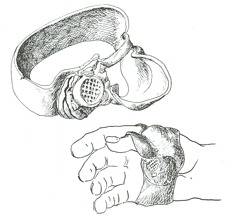
\includegraphics{images/sejlskibe_tema-2-sejlhandsk.png}
\caption{Sejlhandsker til at beskytte hænderne mod slid.}
\end{figure}

\sFram{showBlue}{
    \subsection{Merlespiger}
Merlespigeret var en aflang spids lavet af metal eller træ. Merlespiret var en naturlig del af sømandens udstyr. Merlespiger blev brugt til at splejse tovværk, det vil sige at sætte forskellige stykker tovværk sammen, så man kunne få den rigtige længde. Man splejsede også tovværk, hvis man skulle indsætte et øje – altså et hul eller en ring, man kunne trække noget igennem eller hægte noget fast i. Splejsning kunne også bruges til at forstærke tovet med.
    \subsection{Sejlhandsker}
Sejlhandskerne var lavet af læder og beskyttede hånden mod slid. Man brugte handsken, når man skulle sy et nyt sejl eller reparere sejl, der var gået i stykker. På sejlhandsken var der indsyet en brik, som støttede nålen. I land var det at være sejlmager et erhverv, mens det på skibene oftest var de ældre matroser, der fungerede som sejlmagere.
}

Udrustningen blev der mange gange sørget for hjemmefra. Køjesækken og
skibskisten var vigtige. Skibskisten blev gerne pakket af moderen. Og
konfirmanden kunne regne med at få en god og fornuftig udrustning med
sig med tøj til alt slags vejr, hvis familien var vant til at beskæftige
sig med arbejdet på søen. Selve mønstringen om bord foregik på den måde,
at den nye dreng fik anvist en køje forude - og så blev han straks
kastet ud i arbejdet. Allerede på det tidspunkt gik sølivets barske
realiteter op for den unge, og nogle af barndommens drømme er nok
hurtigt fordampet op i den blå luft.

\begin{figure}
\centering
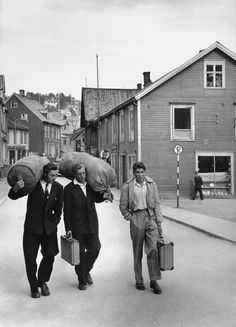
\includegraphics{images/sejlskibe_tema-2-koejesaek.jpg}
\caption{To sømænd med deres køjesække over skulderen.}
\end{figure}

\sFram{showBlue}{
    \subsection{Køjesæk}
Køjesækken var en lærredssæk med ringe slået i foroven, så den kunne snøres sammen. Sommetider malede ejermanden sit navn på sækken, så han lettere kunne kende den. Andre malede billeder på sækken – f. eks. to krydsede flag. Køjesækken blev brugt til at opbevare sømandens dyne, hoved-pude, dynebetræk og undertøj. Det var det, man kaldte for ”køjetøjet”. Ikke alle søfolk havde råd til en dyne, så de måtte nøjes med et tæppe.
}

\chapter{Høj og lav}

\emph{''Der var mange gange, at skipperen eller styrmanden sagde til
drengene: ''Nu ka' I bare vente jer til vi kommer i søen, så skal vi nok
sørge for jer!'' Se det var jo en trussel, at så skulle de have tæsk, og
så var det vel årsagen mange gange til, at de simpelthen bare stak af
for at blive fri for skibet.''}

\begin{figure}
\centering
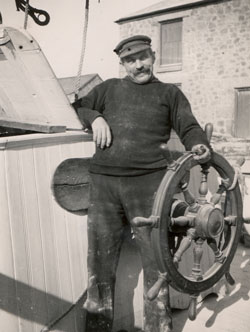
\includegraphics{images/sejlskibe_tema-3-skipper.jpg}
\caption{Skipper på et sejlskib.}
\end{figure}

Livet på sejlskibene var underlagt en lang række love og regler, skrevne
såvel som uskrevne. Mange af disse regler var nok nødvendige, mens nogle
i vores øjne kan virke barske og urimelige. Et sejlskib langt fra havn
var som et afsondret lille samfund, og i tilfælde af krise måtte der
ikke herske tvivl om, hvem der gjorde hvad. Derfor havde
\textbf{skipperen}\footnote{\textbf{Skipperen} er lederen af mandskabet
  på et skib.} eller kaptajnen altid det endelige ord, og man skulle
altid adlyde ham. Det var også skipperen, der var øverste myndighed,
altså en slags dommer om bord. Det var ham, som kunne straffe folk ved
at trække dem i løn eller sætte dem i land i den nærmeste havn. Det gav
skipperen et stort ansvar, men også mulighed for at tyrannisere sine
folk, når skibet var på havet, hvis det var det, han ville. Omvendt
kunne han også belønne mandskabet med ekstra fritid i havn, ekstra kost
eller måske en lønforhøjelse.

Når man stod til søs med et sejlskib, måtte man blot håbe, at skipperen
var en rimelig mand, og at han og besætningen behandlede én godt. Men
det var ofte ikke tilfældet. Selv om det var ulovligt, blev fysisk
afstraffelse som tæv eller spark ofte brugt over for skibsdrengene, der
jo var nye i faget og lavede fejl en gang imellem. Man kunne ikke stille
meget op, hvis man kom om bord på et ''uheldigt skib''. Man var ifølge
loven forpligtet til at sejle med i minimum to år, og der var ikke
mulighed for at sige jobbet op. Stak man af fra skibet, når det kom i
havn, blev man kaldt for ''rømningsmand''. Og hvis man var det, måtte
myndighederne i land arrestere en, og så måtte man betale en ret stor
bøde eller i værste fald gå i fængsel.

\emph{''Jeg mønstrede om bord i en galease, der lå i Frihavnen i
København og skulle være bedstemand. Det var et lille skib -- indenrigs.
Da jeg havde været der i to dage, så pakkede jeg sgu min sæk og så gik
jeg i land. Jeg havde fået 15 kr. i forskud til en ny halmmadras. Så
lagde jeg resten af pengene på madrassen og til ham den anden dreng, der
var om bord, sagde jeg: ''Nu ka' du give ham dem der og sige jeg er
gået!'' Så var jeg jo rømningsmand. -- Men så kom der jo bud fra
\textbf{Sø- og Handelsretten}\footnote{\textbf{Sø- og Handelsretten} er
  en domstol for sager, der har med skibe at gøre.}, at jeg var
rømningsmand og jeg skulle straffes. Og så fik jeg en bøde på 12 kroner,
og ham det frække bæst der i \textbf{Holmensgade}\footnote{\textbf{Holmensgade}
  er en gade i København.} 1. udskrivningskreds han mente jo, jeg var et
forfærdeligt menneske, at jeg sådan kunne rømme fra skibet. Han skrev
ned i min søfartsbog, at jeg rømte. Så tænkte jeg: ''Tak skal du ha', nu
får du aldrig nogen hyre mere!'' Nej, jeg var en storforbryder!''.}

\begin{figure}
\centering
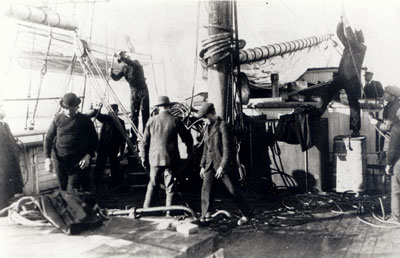
\includegraphics{images/sejlskibe_tema-3-arbejdsfor.jpg}
\caption{Her ses besætningen i fuld gang på et sejlskib. Styrmanden
kigger på til venstre i billedet.}
\end{figure}

Om bord på skibet var folk ordet efter rang. Officererne var
selvfølgelig øverst, men mellem resten af mandskabet var der nogle helt
klare, uskrevne regler for, hvordan man skulle omgås hinanden. Der var
ingen plads til sarte følelser eller fine fornemmelser. Omgangstonen var
rå og kontant, men sammenholdet kunne være stærkt.

De ældste matroser havde mest at skulle have sagt. Den ældste fik den
bedste køje og det behageligste arbejde, men måtte til gengæld gå
forrest, når det virkelig gjaldt. Det kunne være vanskeligt arbejde i
\textbf{riggen}\footnote{\textbf{Riggen} er alt det, der sidder på
  masterne.} eller måske som søfolkenes talsmand over for kaptajnen,
hvis der var noget, de var utilfredse med. Systemet fortsatte hele vejen
ned til skibsdrengen eller kokkedrengen, der ikke havde ret meget at
sige. Til gengæld var det almindeligt, at man skulle hjælpe hinanden med
arbejdet og hverdagens problemer. Den mere erfarne skulle være parat til
at hjælpe den mindre erfarne med arbejdet.

\begin{figure}
\centering
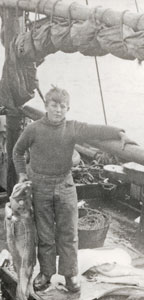
\includegraphics{images/sejlskibe_tema-3-skibsdreng.jpg}
\caption{En skibsdreng om bord på et sejlskib.}
\end{figure}

\sFram{showBlue}{
    \subsection{Skibsdreng}

Nederst i hele skibssamfundet stod drengene. Det var de nykonfirmerede knægte, der udmønstrede som skibsdrenge. Skibsdrengens opgave var at gå til hånde ved alt arbejde, at gøre rent forude og agterude, vaske og spule. I logaret eller lukafet, der var et lille opholdsrum ude foran under dækket, skulle han hjælpe til med at hente maden i kabyssen, tage af bordet og vaske op. Det var ikke kun styrmænd og skonnertskippere, som uddelte øretæver. Det gjorde matroser også. Jo, de mest udsatte var de yngste om bord – herunder skibsdrengen.

\emph{”Sommetider da fik jeg jo en øretæve. Det var en matros, der sagde: ”Når vi spiser, og du kan se, vi mangler noget, så skal det ikke siges til dig, at du skal gå hen og hente det, hvis der er mere!” Men jeg sad jo alligevel og lurede – Gud ved om de kan spise mere. Men så rejste han sig bare op, og så smak han mig en. Så kunne jeg nok huske det.”}
}

\emph{''Ja, det er sådan, altså når vi er i søen, at hvis der er et job
vi mener vi kan klare bedre end en anden, at vi ta'r det. Det er somme
tider, det har jeg da set, at de {[}skibsdrengene{]} har stået og rystet
for at skulle gå til vejrs, når sejlet rigtig har slået til. Så har jeg
sagt somme tider: ''Bliv du bare nede, det skal jeg nok klare selv.''
Det har jeg gjort flere gange. Og jeg ved en jeg sejlede med, senere han
blev skipper, da jeg kom til at sejle med ham, så sagde han: ''Jeg kan
sgu huske da jeg var en dreng, du var flink ved mig og lod mig blive
nede.'' Men jeg vidste jo, hvor farligt det var for nybegyndere at komme
op i sådan et sejl.''}

\begin{figure}
\centering
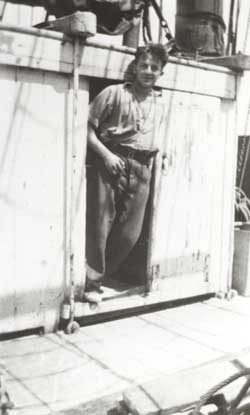
\includegraphics{images/sejlskibe_tema-3-kokkedreng.jpg}
\caption{En kokkedreng om bord på et sejlskib.}
\end{figure}

\sFram{showBlue}{
    \subsection{Kokkedreng}

I skibe, der sejlede med op til 6 mands besætning, havde man hyret en kokkedreng til arbejdet i kabyssen. Han blev som regel kaldt ”kok”. Til kokkedreng valgte skipperne gerne den mindste og svageste dreng. En sømand, som var lille af vækst, kunne have vanskeligt ved at udmønstre som letmatros eller matros, men som kok gik det bedre an.

Stillingen som kokkedreng var dog ikke attraktiv for de unge, blandt andet fordi kokken skulle være flere steder på en gang. Dels skulle han sørge for kabyssen, dels skulle han deltage i alt andet forefaldende arbejde. Heldigvis havde mange mødre givet sønnen et hurtigt kursus i madlavning, inden han skulle til søs som kokkedreng. Det var desuden almindeligt, at skipperen eller styrmanden gav drengen gode råd og vejledning i arbejdet, fordi besætningen ellers kunne risikere at få uspiselig mad.
}

Folkene holdt øje med hinanden i dårligt vejr og var parat til at give
en hånd, når det kneb. Det var en helt naturlig sag, og der var ingen,
der sagde tak for hjælpen -- man forventede, at alle ville gøre det
samme. En selvfølge var det, at man deltes om
\textbf{provianten}\footnote{\textbf{Proviant} er maden om bord på
  skibet.}. Der var ingen, der kunne tage noget til side til sig selv
uden at være en dårlig kammerat. Derfor købte man heller aldrig ekstra
proviant med. Man hjalp også hinanden i fritiden, og at låne lidt penge
til en kammerat var der ikke noget i vejen for.

''Hvis der var noget man kunne hjælpe med gjorde man det. Jeg har da
f.eks. vasket tøj for en og syet og stoppet for en anden -- en svensker,
og jeg blev selv engang hjulpet med nogle rubler oppe i \textbf{Skt.
Petersborg}\footnote{\textbf{Skt. Petersborg} er en by i Rusland},
dengang kunne jeg ikke få noget hos skipperen. Der var en der gav mig
lidt. Han tænkte det var synd, at jeg ikke skulle have en ting med hjem
til mine forældre. Man kunne købe de her æg med mange små inden i og
tobaksdåser. Det var russisk lakarbejde.''

\sFram{showBlue}{
    \subsection{Proviant}
Proviant var et andet ord for den mad og drikke, som skibet skulle have med sig, når det stod ud på rejse. De skibe, som udrustede sig til årets togt eller måske flere års togt, havde om foråret travlt med at ordne provianteringen. Så vidt muligt provianterede man i sin hjemby. Her kendte man priserne, og folk vidste, at det ikke kunne betale sig at snyde en lokal kunde. Tit var det sådan, at et par eller flere af handelsfolkene havde andel i skibet, og så gik man naturligvis først til dem og handlede.

Købmanden fik sin bestilling, og det samme gjorde slagteren og bageren. Alt det indkøbte blev omhyggeligt noteret i regnskabet. Man ville ikke bruge for mange penge på kosten. Efterhånden kom det så om bord, æg og margarine, rugbrød, kød og flæsk, fisk, sild, grøntsager, mælk, gryn, kartofler osv. Man havde ikke køleskab, så kødet blev saltet i tønder. Var man længe til søs, blev nogle af madvarerne ofte fordærvede. Man provianterede derfor også undervejs på rejsen, hvis man havde mulighed for det.
}

\begin{figure}
\centering
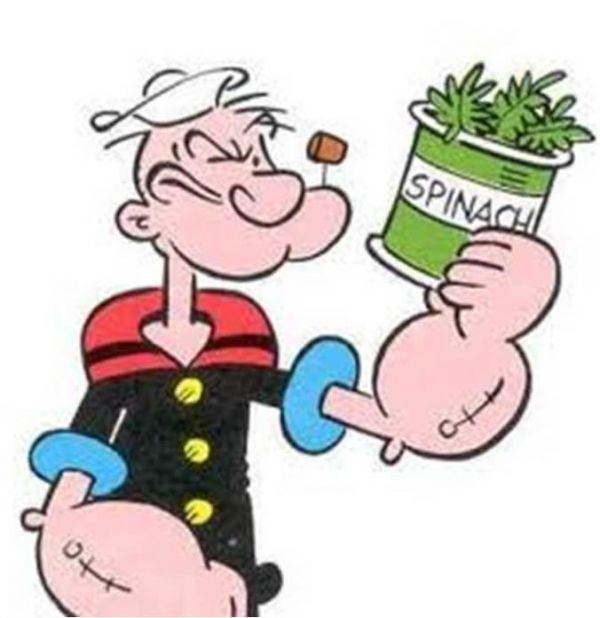
\includegraphics{images/sejlskibe_tema-3-proviant.jpg}
\caption{Provianten om bord på skibet kunne variere meget.}
\end{figure}

Gensidig tillid var forudsætningen for, at man kunne hjælpe og stole på
hinanden som skibskammerater. Hvis nogen brød denne tillid, reagerede de
andre. Tyveri var groft brud på kammeratskabet -- ja, selv mistanke om
tyveri kunne ophidse gemytterne. At låse sin
\textbf{skibskiste}\footnote{\textbf{Skibskister} er en kiste til
  opbevaring af private ejendele som tøj mm.} var det samme som at
beskylde kammeraterne for at være tyvagtige. Den slags tolererede man
ikke.

''Man måtte ikke låse sin skibskiste. Det var det samme som at vi
mistænkte kammeraterne for at stjæle. Jeg havde en lås i kisten, og jeg
kunne ikke tage nøglen ud uden at jeg skulle låse den, og den måtte ikke
sidde i for de stødte benet imod. ''Hvad skal jeg gøre?'' spurgte jeg.
''Ja, du kan brække låsen af!'' sagde de. Det måtte jeg så gøre''.

Bonde var et skældsord i et sejlskib. Et bondeskib var et skib, hvor
tingene blev grebet forkert an, og hvor kammeratskabet ikke fungerede. I
de fleste skibe fungerede kammeratskabet godt. Det betød ikke, at folk
ikke kunne blive uvenner, men konflikterne blev løst efter reglerne. En
af reglerne kunne være slagsmål, helst overvåget af andre af
besætningen. Når kampen var slut, skulle de to kamphaner være gode
venner igen. Der var ikke plads til langvarigt had på et sejlskib, fordi
man var meget afhængige af hinanden.

\chapter{Lev vel?}

\emph{''Efterårsdage blev vi aldrig vasket i søen. Heller ikke om
vinteren. Det var alt for koldt at tage noget tøj af og stå der og vaske
sig. Det kunne man ikke. Sommerdage der på Østersøen kunne vi jo tage
udenbordsvand.''}

\begin{figure}
\centering
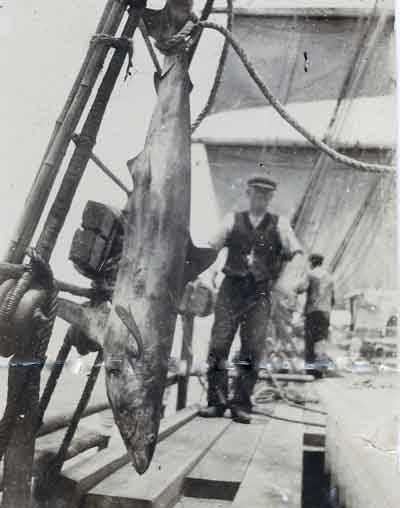
\includegraphics{images/sejlskibe_tema-4-haj.jpg}
\caption{Frisk fisk var et velkomment supplement til kosten. Her ses en
friskfanget haj et sted i Atlanterhavet på skonnerten Kodan.}
\end{figure}

Hverdagen på et sejlskib kunne være hård. Arbejdet var krævende, og de
hygiejniske forhold ikke for gode. Man boede trangt, kunne ofte ikke
komme i bad, og kosten var sparsom. Madlavningen foregik i et lille
aflukke \textbf{(kabyssen)}\footnote{\textbf{Kabyseen} er køkkenet om
  bord på et skib.} placeret midt på dækket, hvor der lige var plads til
at vende sig. Maden blev lavet på et lille komfur, hvor røgen let kunne
slå ind og fylde rummet. Det var heller ikke altid nemt at lave mad, når
skibet gyngede kraftigt i en storm eller en forkert sø. Madlavningen på
de mindre sejlskibe blev som regel altid foretaget af yngste mand
ombord. På de mindste skibe kunne det være forbundet med hårdt arbejde.
Foruden madlavningen skulle kokken også hjælpe til med alt det andet om
bord. Om vinteren kunne det dog have sine fordele at være i kabyssen.

\emph{''Kabyssen var det eneste sted der var varme. Der var ikke varme
nogen steder om vinteren undtagen kabyssen. Det var det eneste sted vi
kunne få tørret et par strømper.''.}

Kosten var meget forskellig fra skib til skib. Meget afhang af, om
kokken kunne lave god mad ud af den proviant, man havde med i skibene.
På nogle skibe spiste man godt, mens der på andre blev sparet på kosten.
Når først skibet var afsejlet, kunne man ikke gøre så meget.

''Der var meget forskel på det. Ja -- uha. Nogle var hele
\textbf{sultekasser}\footnote{\textbf{Sultekasser} er skibe, hvor man
  fik for lidt at spise.} og andre var nogenlunde. De sparede på kosten
for at give rederiet mere. Det var jo om at få overskud på de skibe. Jo
mere de sparede på kosten jo mere tjente de jo for pokker. Vi kunne godt
klage, men når vi ikke havde ud-provianteret mere og lå i søen, så var
man nødt til at indordne sig.''.\_

Frisk kød var en sjældenhed. De store skibe, der krydsede oceanerne,
havde dog ofte levende grise om bord. Der var også mulighed for at
supplere kosten med fiskefangst. Fik man harpuneret en haj eller en
delfin, kunne man være heldig at få helt frisk kød. Dårlig eller for
lidt kost kunne føre til mangelsygdomme og svække immunforsvaret. Og det
kunne være farligt, når man kom til byer, hvor der var udbrudt epidemi.
\textbf{Kolera}\footnote{\textbf{Kolera} er en smitsom mave-tarm-sygdom,
  som ofte dukker op i forbindelse med urent drikkevand.},
\textbf{dysenteri}\footnote{\textbf{Dysenteri} er en smitsom
  tarmbetændelse med blodig diarré. Opst som følge af dårlig hygiejne i
  troperne.}, \textbf{tyfus}\footnote{\textbf{Tyfus} er en art af
  blodforgiftning og den farligste af alle salmonelleinfektionernen.
  Opstår som følge af forurenet mad og drikke i troperne.} og lignende
skavanker var kendte fænomener blandt søfolkene. Alle frygtede at blive
syge. Tænkte man sig ikke om, kunne det betyde, at man måske døde.

\emph{''I Petersborg stod vi og \textbf{handede}\footnote{\textbf{Handede}
  betyder `rakte', eller `videregav'.} sten. Så havde vi godt nok fået
at vide, at der var kolera. Vi måtte endelig ikke gå i vandet. Vi havde
jo jollen liggende i vandet agterud, og når så vi havde stået og handet
næsten op fra lasten og op i land fra 6 morgen til 6 aften og svedt, og
det var egentlig hårdt arbejde, så kunne vi jo ikke nære os om aftenen,
andet end at vi skulle lige ned og skylle os en bitte, og der var ingen,
der så det, når vi gik ned i jollen og så blev vasket en bitte. Men det
resulterede alligevel i, at vi havde en tysker om bord fra Königsberg,
og han fik kolera og blev lagt i land og han døde dèr. Vi skulle jo have
holdt os væk, men vi andre, vi gik da fri.''.}

En anden plage var \textbf{søsygen}\footnote{\textbf{Søsyge} opstår som
  følge af ubalance i balancesansen. Kendetegn er kvalme, depressiv
  tilstand, opkast og mavesmerter.}, som naturligvis var en del af
sømandslivet. De fleste søfolk havde på et eller andet tidspunkt oplevet
søsyge. For nogle var det en konstant plage, mens søsygen for andre var
et engangsfænomen. En slem søsyge kunne tage modet fra de fleste.

\emph{''Om sommeren lastede vi kridt til Kotka, og det blev dårligt
vejr. Vi lå underdrejede oppe i bugten ved Øland. Jeg mener vi lå der i
halvandet døgn, og drengen var så søsyg, så ganske forfærdelig søsyg, og
han lå og rullede rundt i vandet. Det var frygteligt at se. Vi fik så
meget vand over, at vi næsten ikke kunne komme ned i forlogaret. Så
sagde jeg til skipperen: Nu lægger jeg ham ned i min
\textbf{køje}\footnote{\textbf{Køjer} er senge om bord på et skib.}. Ja,
han ville ikke have ham derned og brække\ldots{} Jamen han har ikke
noget at brække af, det kan du godt tro. Han kom så med der. Så lå han
dernede en dags tid. Han var aldrig søsyg mere.''.}

Bedre blev det heller ikke af, at toiletforholdene var meget primitive.

\emph{''Ja, se vi havde en lille tønde, f.eks. styrmand og skipper de
havde jo henne i hytten agter, der havde de jo en spand, og den skulle
kokken jo holde, sørge for at tømme hver anden dag. Men mandskabet
forude, de havde jo bare en rund tønde med to stropper i, og når vi så
lå i havn, så skulle de sørge for at krybe i læ et eller andet sted,
særlig hvis der gik damer på kajen. Der var i hvert fald tønde, og så
fyldte vi en halv spand vand i og så ud over siden med det. Men altså,
vi havde ikke andet end den åbne tønde.''.}

Hvis sejlskibet var af ældre dato, kunne det være plaget af småkryb. Den
erfarne sømand vidste, at det var bedst at holde sig væk fra skibe med
skadedyr, hvis man kunne.

\emph{''Det var meget almindeligt dengang med sådan utøj om bord. I
\textbf{barkentinen}\footnote{\textbf{Barkentine} er en skibstype med
  mindst tre master.} \textsc{Haabet} her af byen var der mange
væggelus. Jeg var mønstret i den og skulle med den ud at sejle. Så var
de andre kommet om bord, men jeg sov jo hjemme. Først lå de i køjerne,
så lå de på deres \textbf{kistebænke}\footnote{\textbf{Kistebænke} er
  kister, man kunne sidde på.}, og så gik de i land. Så sagde jeg til
kaptajn Andersen: Ja, nok er jeg mønstret her, men jeg er nu ikke
\textbf{mønstret}\footnote{\textbf{Mønstre} er at gå om bord og få hyre
  på et skib; det er altså begyndelsen på jobbet.} til at være sammen
med sådan en besætning som den der, så jeg vil i land. Åhr, det kunne
jeg altså ikke komme. Ja, det vil jeg altså, for jeg vil ikke sejle
sammen med alle de væggelus. Noterne mellem plankerne de var helt røde
af bare lus. Men der var masser af skibe, der havde væggelus dengang, og
man kunne gerne se det ved at lyset brændte på de skibe om natten for at
holde lusene lidt i ave. Så kom jeg ikke med den.''.}

\emph{''Kakerlakker det var jo nogle bæster. Når vi skulle sove så
rendte de jo og kneb os, men det var ikke farligt på nogen måde. Men se
der i sejlskibene, selv om der var kakerlakker og væggelus, så blev det
jo ikke røget ud som f.eks. i damperne. De skulle have bevis. Det måtte
ikke blive over 6 mdr. gammelt, og hvis der var utøj om bord, så skulle
skibet svovles hver 6. måned. Så blev vi jaget i land nogle timer.''.}

\chapter{Sjov og alvor}

\emph{''På frivagterne om bord i søen da sov vi jo den meste tid. Somme
tider spillede vi kort. Noget skulle tiden jo gå med.''}

Fritid til søs var der ikke meget af i sejlskibene. I gennemsnit havde
man 12 timers arbejde og 12 timers fri i døgnet. Med et almindeligt
søvnbehov på 7-8 timer var der kun 4-5 timer i døgnet til at spise,
klæde sig på, drikke te eller kaffe, personlig hygiejne samt
toiletbesøg. For det meste blev fritiden sovet væk -- der var ikke tid
og kræfter til andet.

\emph{''\textbf{Frivagterne}\footnote{\textbf{Frivagter} er fritid om
  bord.}? Puh-ha. Der røg vi lige på hovedet i køjen og så sov vi lige
som en sten.''}

Søfolkene var på mange områder afskåret fra omverdenen. Der eksisterede
ingen form for radio, ingen nyhedsinformation, ingen underholdning -- ud
over hvad de selv kunne finde på. Når skibet var i søen, betød det
mindre. For det meste nåede man kun lige at stikke hovederne sammen
ganske kort, inden der skulle soves. Og tit var der kun tid til at læse
eller genlæse breve hjemmefra. Egentlig fritid om bord kunne man stort
set kun opleve på de store \textbf{fuldriggede sejlskibe}\footnote{\textbf{Fuldriggede
  sejlskibe} er skibe med råsejl (firkantede sejl) på alle master.}, der
med passat-vindene i ryggen krydsede de store oceaner.

\emph{''Som regel der i de danske skonnerter når de havde frivagt, og de
havde været oppe og havde puklet i den tid, så var de sgu gerne så
udmattede, så de sov altså fra det hele. Så var det en anden ting i de
store sejlskibe i \textbf{passaten}\footnote{\textbf{Passatvinde} er
  jævne vinde, der blæser hen over verdenshavene.}, hvor det var så fint
vejr, der var mange der brugte deres frivagt til at lave skibsmodeller
-- helmodeller eller halvmodeller og andre sådan forskellige ting.
Ligesådan flaskeskibe blev der lavet. Jeg kan huske flere gange jeg var
på Charlie Brown, en meget kendt beværtning i London, hvor alle verdens
søfolk kom når de havde mønstret af, og der var alting deroppe -- der
var krokodiller og assagaier og alt mellem himmel og jord og
skibsmodeller, og der var det så tit, når søfolkene ikke havde mere, så
tog de sgu deres skibsmodel under armen og gik op og sagde, hvad kan jeg
få for den? Jah, du kan få \textbf{ti shilling}\footnote{\textbf{Shilling}
  er en engelsk møntenhed. Svarede til 4 kroner, og det er ca. 90 kroner
  i dag.}, og så kan du indløse den. Og så fik de ti shilling og drak
dem op, og den blev aldrig indløst, så de fik jo nogle souvenirs --
folks arbejde der.''}

\emph{''I skonnerterne var der ikke noget fritid. Men i de store skibe.
Jeg kan huske engang vi lavede sådan en kludebold. Dagen før havde der
været åbent i \textbf{slopkisten}\footnote{\textbf{Slopkisten} er
  kaptajnens lille private butik om bord.}, og så var der en af mine
kammerater, en matros der havde købt et par sko, og dem havde han på
dagen efter, da vi spillede fodbold. Vi løb rundt på stordækket og det
havde jo ikke meget med fodbold at gøre. Det var nærmest sådan tjatteri.
Og så sparkede han kraftigt, så denne her sko røg af og op i rigningen
og \textbf{udenbords}\footnote{\textbf{Udenbords} vil sige vandet, der
  omgiver skibet.} regnede han med. Der røg din sko udenbords, var der
nogen der råbte. Ad helvede til, råbte han, så blev han så gal, så tog
han den anden af og smed ud. Men så var der en der sagde -- jamen her
sidder jo din sko -- den sad fast i rigningen. Så blev han endnu mere
tosset.''}

\begin{figure}
\centering
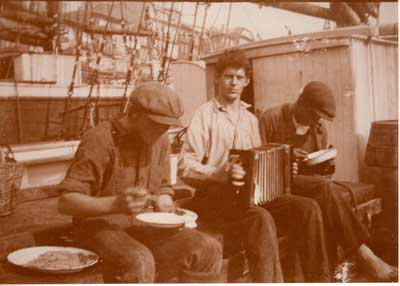
\includegraphics{images/sejlskibe_tema-5-spisning.jpg}
\caption{Der spises et måltid mad til lidt musik mens skibet er i havn.}
\end{figure}

Det hændte, at der blev spillet musik og sunget, men som regel ventede
man til skibet kom i havn. Det var i havnene, sømændene kunne slå sig
løs, mens skibet ventede fragter eller skulle repareres. Når skibet
nærmede sig en havn efter mange dage til søs, begyndte landgangsfeberen.
Snakken tog til om alle de ting, man skulle nå, inden sejladsen blev
genoptaget. Nogle brugte straks opholdet i havnen til at få et
velkomment kosttilskud.

\emph{''Når vi kom til en dansk havn, så røg vi op og købte en hel
lagkage. Den kostede 2 kr. -- en flødeskumslagkage. Så åd vi den. I
England købte vi plumbudding, og i Spanien købte vi engang nogle fine
kager, og der var noget i, og det var sgu klipfisk, så vi åd dem altså
ikke. Vi havde lige losset klipfisk og så få en kage med klipfisk!''}

Sømændene var afskåret fra et almindeligt seksualliv. I uger og måneder
lå de ude til søs uden at have kontakt med kvinder. De unge var afskåret
fra at søge den naturlige kontakt til jævnaldrene unge piger, og de
voksne mænd måtte undvære deres kæresters kærlighed. I det mandssamfund,
som skibene udgjorde, blev kvinder for nogle en besættelse, og besøg i
havn kunne ikke råde bod på den manglende kontakt med kvinder. Disse
havnebesøg blev for det meste et spørgsmål om hurtigt at tilfredsstille
nogle seksuelle drifter -- det vil sige, at man købte sig til et samleje
med en totalt fremmed og uvedkommende pige, for hvem det kun gjaldt om
at få det overstået. Allerede mens skibet var på vej ind, havde man om
bord besluttet sig for, om man skulle på bordel eller horekasse, som man
også kaldte det. En ung sømand, som tøvede med at slutte sig til
selskabet, kunne blive til grin blandt de andre.

\emph{''Jah, når søfolkene de gik i land -- hvis der var bordeller, så
gik de ind på dem og ellers på havnerestaurationer, hvor de kunne træffe
piger. Det var gerne de ældre som tog føringen. Vil I med derhen? Skal
vi det i aften? Og sådan. Nogle ville jo med og andre ville ikke. Der
var ingen tvang, men sådan en ung mand som ikke ville med på bordel
kunne de godt lide at drille lidt -- åh -- sådan en barnerøv osv. Så
hændte det jo, at han til sidst tænkte \(\ldots\) det skal de skisme
ikke tro \(\ldots\) og gik med.''}

Frygten for kønssygdomme afholdt dog nogle fra at gå med.

\emph{''Der var en fisker med oppe fra \textbf{Hanstholm}\footnote{\textbf{Hanstholm}
  er en fiskerby i Nordvestjylland.}. Vi kom til
\textbf{Malaga}\footnote{\textbf{Malaga} er en havneby i Sydspanien.} og
skulle \textbf{losse}\footnote{\textbf{Losset} er, når varerne er kommet
  ud af skibet.} fisken, og så var han gået op til nogle piger, og så
gik han og ragede sig en gonoré til, og jeg så hvordan han skabte sig og
jamrede sig, og han blev lagt i land på et hospital og kom slet ikke med
skibet, vi måtte sejle fra ham. Da tænkte jeg ved mig selv: For det
første kom jeg fra et godt barndomshjem, og for det andet, tænkte jeg,
du skal aldrig komme til sådan en pige, for der er alligevel risiko, når
jeg havde set ham, hvordan han led og så blev sejlet agterud dernede i
Malaga, så tænkte jeg ved mig selv: nej, det skal du holde dig fra!!'' }

Nogle prioriterede i stedet det at komme ud at se noget nyt. Det kunne
være tyrefægtning i Spanien, en tur i teatret i London eller måske noget
helt tredje.

\emph{''Jeg kan huske, da vi lå i Norge, da var vi ude at se på
Holmenkollen -- nej, det med værtshuse, det har jeg ikke haft lyst til
sådan.''}

\chapter{Pas På !}

\emph{``\textsc{Primo} forsvandt i \textbf{Nordatlanten}\footnote{\textbf{Nordatlanten}
  er havet mellem Norga, England, USA, Canada og Grønland.} lige efter,
at jeg var gået fra den. Det var en 3-mastet skonnert. Jeg kom i land på
\textbf{Københavns red.}\footnote{\textbf{Københavns red} er det sted
  uden for havnen, hvor skibene lå for anker.} Så rejsen efter, da
forsvandt skibet. Ja, de fandt den senere, men de fandt aldrig
besætningen.''}

\begin{figure}
\centering
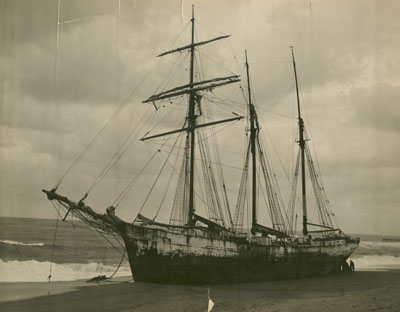
\includegraphics{images/sejlskibe_tema-6-forlis.jpg}
\caption{Mange sejlskibe blev med vilje sejlet ind på land, hvis
mandskabet frygtede forlis. \{3\}}
\end{figure}

Når man satte sine ben i et sejlskib, udsatte man sig også for en vis
risiko. Man blev ganske vist rig på oplevelser, men kunne også i værste
fald miste livet. Farerne lurede. Sygdom, lemlæstelse eller død var
noget, de fleste søfolk stiftede bekendtskab med på et eller andet
tidspunkt i deres karriere. De hørte om skibe, der forsvandt, mødte
kolleger, som døde af feber, eller oplevede måske selv en ulykke, som de
mirakuløst overlevede. Det var ikke ualmindeligt, at gamle matroser
havde oplevet indtil flere \textbf{forlis}\footnote{\textbf{Forlis} er,
  når et skib snak eller på anden måde gik i stykker.}, som de med gru
kunne fortælle om nede i logarets mørke. Grumme historier var en
uundgåelig del af sølivet, og det var ikke uden grund, at søfartssamfund
havde en større andel af enker end andre steder. Et sejlskib var ganske
enkelt en af de farligste arbejdspladser, der fandtes. Det frygtede råb:
''Mand overbord!'' betød i dårligt vejr for det meste et farvel til en
skibskammerat, der blev overladt til den ensomme druknedød. Voldsomme
oplevelser kunne føre til syner eller en stærk tro på større magter.
Troen på Gud kunne være stærk, men afhang også af det hjem, som sømanden
kom fra. Nogle var mere troende end andre.

\begin{figure}
\centering
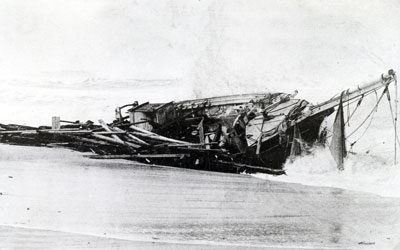
\includegraphics{images/sejlskibe_tema-6-vrag.jpg}
\caption{Vrag af sejlskibet Castor, der strandede ved Casablanca i 1913}
\end{figure}

\emph{''Jeg stod henne ved skipperen, han stod ved roret og havde
\textbf{sejsing}\footnote{\textbf{Sejsing} er tovværk, man bandt om
  sejlene.} omkring livet, og så siger han, ''hold dig ved'', siger han,
''for der kommer en grim \textbf{sø}\footnote{\textbf{Sø} er en eller
  flere bølger.}'', og så kiggede han ud til siden, men vi skulle kigge
opad, da kom den rullende oppe over os, lige som sådan en elektrisk pæl
der er i højden, og så faldt den jo i øvrigt, og jeg tog fat under
\textbf{ruffet}\footnote{\textbf{Ruffet} er dækhuset, der benyttes til
  kahytsrum.} sådan og jeg har sørme taget sådan, at mine negle de var
gået ind i træet. Men der var ikke noget at gøre, jeg blev væltet ud, og
jeg havde som ærlig talt troet, at jeg var druknet, det troede jeg. Alt
var jo mørkt, når man kom under sådan en masse vand, men det har jo
været mit held mange gange, at jeg har været udsat for det og er sluppet
godt fra det.}

\emph{Ja, jeg blev faktisk smidt lige på hovedet ind på dækket, og så
var jeg på vej ud igen, men så tog skipperen mig så. Og da kunne jeg
høre, det er altså sådan noget, man får i øjeblikket, jeg hørte en
koncert af den skønneste musik, som du kan tænke dig, og i min
underbevidsthed, dèr var jeg klar over, at jeg tænkte, jeg vidste ikke
rigtig, hvor jeg var henne, jeg var slet ikke klar over, om jeg i det
hele taget levede, men jeg hørte denne her musik, og så lige pludselig
hører jeg nogen, der siger: ''Lever du, er du vågen'', og så var det
skipperen, der stod og ruskede i mig. Og så vågnede jeg op, og så siger
han ''Fejler du noget''. ''Nej, jeg gør ikke'', siger jeg så, da var jeg
ved at være rask. Så siger han, ''Så gå hen og hjælp til med at hale det
sejl ned''.}

\begin{figure}
\centering
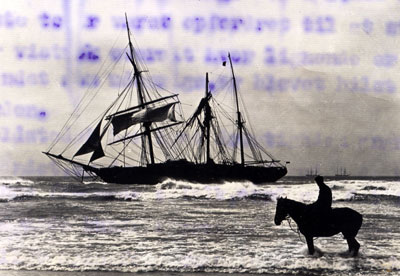
\includegraphics{images/sejlskibe_tema-6-strandet-s.jpg}
\caption{Strandet skib}
\end{figure}

\emph{Og det var det sejl, at søen havde splintret alle trådene der. Der
var jo tusinde tråde og det var det, at stormen fløjtede i, og det var
det, der lavede musikken jo. Og så står jeg derhenne sammen med mine
kammerater, og jeg så med det samme, vi mangler en mand, men jeg kunne
ikke sige, hvad han hed. Det kunne jeg ikke.}

\emph{Men, - så gik jeg hen og sagde til skipperen ''Vi har mistet en
mand'', og med det samme han sagde ''Det er Hans'', da var jeg klar over
det. Nej, der var ikke noget at gøre ved det. Ja, så sagde skipperen,
jeg skulle kravle et stykke op i rigningen og kigge, og skønt der lå
planker og brædder her og der, kunne jeg ikke undgå at se han lå og
fægtede med armene, men -- ak gud fader, der var ikke noget at gøre
\(\ldots\) (bevæget). Nej, ok nej, - vi var selv så hjælpeløse, selv om
vi havde villet, ku' vi ikke ha' drejet den, eller fået den til at køre
rundt. Det ku' vi ikke. Så havde vi skullet bruge flere kilometer. Det
kunne vi ikke. Det sagde han jo også til skipperen, han bad jo en bøn
for ham, men..''.}

Blandt besætningerne var sygdom altid frygtet. Noget af det værst
tænkelige for en sømand var, hvis han blev sat i land på grund af sin
sygdom på et hospital og derefter agterudsejlet -- det vil sige, at
skibet sejlede sin vej med den raske besætning. Skete det i troperne,
var man nærmest prisgivet. Risiko for følgesygdomme kombineret med
mangelfuld pleje gjorde, at særlig mange døde på de kanter. Nogle gange
var sømanden også afhængig af kontante midler. Ingen penge -- ingen
behandling. Om bord var der ikke meget, man kunne stille op. Skipperen
og styrmanden havde ganske vist lidt lægelig viden med fra
navigationsskolen, men når det kom til stykket, kunne de ikke stille
meget op. Småskavanker kunne dog klares med lidt opfindsomhed.

\emph{''Joh, jeg havde tandpine. Hold kæft! Jeg kunne springe overbord.
Ja, jeg havde det hele vejen over Atlanterhavet, jo. Jeg havde ikke mere
forstand på tandpine end som der var honning i en skruptudse. Hvergang
jeg kom op på dækket så var der aldrig noget i vejen. Når man skulle ind
og sove og mente, nu har jeg det dejligt, så lige så snart jeg lagde
hovedet på hovedpuden, så havde jeg tandpine med det samme. Jeg havde
det sådan, at jeg var ligeglad med hvad jeg gjorde! Til sidst så glødede
jeg en \textbf{sejlnål}\footnote{\textbf{Sejlnål} er en nål til at sy
  sejlene med.}! Kokken han sagde: ''Må jeg stikke den ned?'' Gu' må du
ej, den vil jeg sgu selv hav lov at stikke ned.'' Jeg fik lige fat i den
-- han skulle kigge mig i munden om det var rigtigt -- så jagede jeg
til. Men jeg tror nok, jeg sprang helt ''op over fokkeråen''! Hold da
kæft hvor gjorde det ondt! Så var den tandpine væk. Jeg havde brændt
nerven over.}

\emph{Men da havde jeg så også gået med det i over en måned. Og jeg
stoppede papir i ørerne, og jeg var lige ved at stoppe \textbf{Social
Demokraten}\footnote{\textbf{Social Demokraten} er en avis.} op i
r\o ven. Ja, hvad jeg ikke gjorde altså, Alt muligt prøvede jeg! Jeg
stoppede sølvpapir ind i ørerne og stoppede det alt for langt ind, så
jeg næsten ikke kunne få det ud igen. Hver nat kl. 12, så kom det. Så
havde skipper fået fat i en \textbf{passer}\footnote{\textbf{Passer} er
  et instrument til at måle afstande på et søkort.} og havde lavet sådan
et par kroge og så snuppede han tanden til sidst. Men han var mindst 8
dage om at få fat i den, den blev siddende.''.}

\chapter{Den store verden}

\emph{``Jeg havde mange sjældne \textbf{konkylier}\footnote{\textbf{Konkylie}
  er en art sneglehus dannet af rovsnegl, der lever i vandet og spiser
  ådsler, mindre fisk og muslinger.} nede fra
\textbf{Vestindien}\footnote{\textbf{Vestindien} er en øgruppe i det
  Caribiske Hav mellem Syd+ og Nordamerika.}. Og så havde jeg et af de
her jernspyd der var med modhage og pyntet sådan som et tyrefægterne
bruger. Jeg havde da også en harpun. Men det hele forsvandt. Mine brødre
havde gået og solgt det for at få penge.''.}

\begin{figure}
\centering
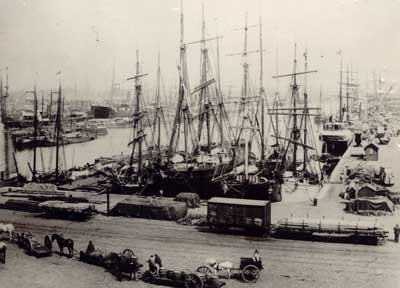
\includegraphics{images/sejlskibe_tema-7-antwerpen.jpg}
\caption{Sømanden havde mulighed for at se verden og møde fremmede
folkeslag. Rejsen til fremmed verdensdele begyndte ofte på en større
europ\ae isk havn som her i Antwerpen i Belgien.}
\end{figure}

De søfolk der fik mulighed for at komme med de større skibe, som sejlede
til andre verdensdele, mødte folk fra helt andre kulturer end den
nordeuropæiske, som de selv var en del af. Dengang havde man et noget
andet menneskesyn end i dag, og fordomme om andre kulturer var
almindeligt. Dog kunne kortvarige bekendtskaber opstå spontant
alligevel, og hvis der var tale om længerevarende havneophold kunne der
knyttes kontakt til de lokale. Lettest var det, hvis der var tale om
andre nordeuropæiske eller nordamerikanske havne. Kom et sejlskib til en
lille havneby, kunne besætningen være så heldig at blive inviteret med
til fest.

\emph{''Vi kom op til New Foundland i december måned. Det var helt sjovt
at komme op og losse kul på sådan en lille \textbf{plads}\footnote{\textbf{Plads}
  er en mindre havn}. Der boede 300 mennesker der. Første dag, vi var
kommet ind, så var der fest. De havde sådan et
\textbf{forsamlingshus}\footnote{\textbf{Forsamlingshus} er et hus, hvor
  mindre lokalsamfund kan mødes til foredrag, fester eller lignende.}
(\(\ldots\)) og når kulskibet kom den ene gang om året, så var der fest,
og det vil sige, at vi jo skulle op og spise til aften, og der kom så de
lokale folk og så spillede de jo. \textbf{Vi stak helt af fra
selskabet}\footnote{\textbf{Vi stak af fra selskabet} betyder herÆ Vi
  lignede ikke de andre.}, for vi havde jo vores sko på og lignede slet
ikke de andre. Men det gik godt og det var sjovt.''}

\begin{figure}
\centering
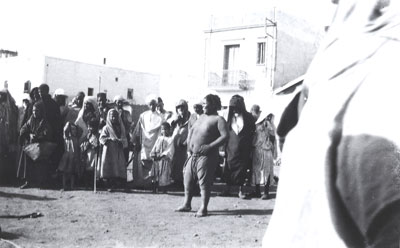
\includegraphics{images/sejlskibe_tema-7-fremmede.jpg}
\caption{Det var spændende at møde fremmede folkeslag}
\end{figure}

Sværere kunne det være for de danske søfolk at begå sig, når de sejlede
til fjerne egne. De folk, som sømændene mødte, var ofte blandt de
fattigste. Det kunne være havnearbejdere, prostituerede eller måske
tiggere, der var henvist til et kummerligt liv i rendestenen. Sprog- og
kulturbarrierer gjorde kommunikationen overordentlig vanskelig.
Alligevel hændte det, at man fik fælles oplevelser med den lokale
befolkning på godt og ondt.

\begin{figure}
\centering
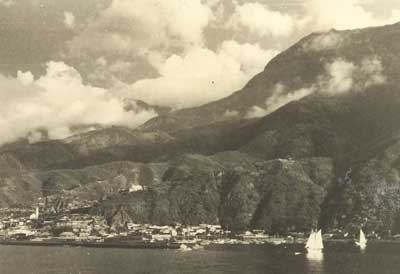
\includegraphics{images/sejlskibe_tema-7-venezuela.jpg}
\caption{Fremmede himmelstrøg, som her en by i Venezuela, satte
fantasien i sving, for hvad mon der ventede i land?}
\end{figure}

\emph{''This, Charles, Hjulemand og jeg omme i floden, som løber ud et
lille stykke herfra, og vaske tøj og hente vand. Fint vand at vaske i.
Vandet har vi nemt ved at få fat i. Vi vender bare båden, så den bliver
næsten fuld af vand, for vi skal jo også være der. Jeg ved ikke hvor
mange mil oppe i landet floden kommer fra, men hele vejen ud bader folk
i den og vasker tøj og smider affald ud i den. Der er ikke meget vand i
den nu. Når vi ligger på maven, stikker ballerne ovenfor. De sorte piger
her har ikke badedragt på, så de må ligge på maven hele tiden. Vi maver
rundt mellem hinanden i al ærbarhed. Det er meget fint drikkevand. Det
kan næsten gå ombord selv, så fyldt af alskens ting er det. Selv hajerne
kan lide det. De kommer helt ind på \textbf{det grunde vand}\footnote{\textbf{Det
  grunde vand} er et udtryk for lavvandet område.}, småhajerne altså,
for at få en god mundfuld af det dejlige vand. Jeg kan gætte mig til,
hvor sprælsk det vil blive, når vi har sejlet rundt i varmen med det i
nogle uger. Når vi så kommer ombord, hiver vi det op med pøse og hælder
det i vandfadene. Vi har to store stående foran \textbf{halvdækket
agter}\footnote{\textbf{Halvdækket agter} er et delvist ovedækket område
  bagerst i skibet.} samt et stort træfad surret på dækket samt en stor
beholder nede i forskibet.}

Traf negeren fra Cape Vincent, vor gode ven. Han gav os kokosnødder. Dem
er der nok af her i træerne. Fik dem i frøkapslen, men han viste os,
hvordan vi skulle få dem ud af den. Vi drikker en del kokosmælk, som
skulle være sundt. Det er i hvert fald rent. Om aftenen var alle mand i
land til fest og fik limonade, men vi gik ret tidligt om bord igen. Det
var en fin måneskinsaften, så Aksel og jeg startede igen. Nu ligger der
en del negerhytter placeret rundt omkring i sandet på vejen op til byen.
I en ret stor, som der ikke var sider i, var der dækket et stort bord
med forskelligt. Der skulle nok være fest, men der var ingen mennesker,
så Aksel og jeg satte os ned og ventede. Der kom ingen, så vi smagte
lidt på varerne, så gik vi, for Sveske blev bange for, at vi skulle få
tærsk, hvis de opdagede os.

Om aftenen til fest på pladsen, ja det er altså en stor plads med træer
og buske. I midten et monument og en åben plads med stole, som vi kan
leje, men det opdagede vi for sent. Det var en aften, alle stolene var
optaget, så rejste et par sig vel for at strække benene lidt, og straks
snuppede vi stolene. De kom tilbage og blev ved at kredse om os, men
sagde ingenting, så vi blev siddende. Senere fortalte Vincent os, at vi
skulle give penge for stolene, så det var en flov historie. Hvad mon
pigerne tænkte om os. Inde på denne lille åbne plads går alle de hvide,
altså noblessen, som vi altså mener vi hører til, idet vi også opholder
sig der. Uden om går så alle de sorte, eller dem som ikke er hvide nok,
og alleryderst går så skravlet.'' .

Indtrykkene fra den store verden tog mange med sig hjem i form af
forskellige souvenirs, der kunne foræres til familien. De hjembragte
sager gjorde som regel altid lykke.

''Nede sydpå havde de alle de sydfrugter, appelsiner og vindruer. Det
var luksus dengang. Jeg købte en stor trækasse med figner. Den havde jeg
med hjem til mine brødre og min søster. De kendte jo ikke andet end de
tørre. Den gjorde lykke den kasse der. Min søster var 1 år ældre end
mig, og hun kunne altid bruge parfume og sådan noget. Det var spændende
med udenlandske ting, især fra Frankrig. Der var ikke så meget ved ting
fra England.''
